% $  Id: validation.tex  $
% !TEX root = main.tex


%%
\section{Validation}
\label{sec:validation}

To validate the appropriateness of CollabIDE, we define two research questions:
\begin{enumerate*}[label=(\arabic*)]
\item Does an automated \ac{VCS} improve productivity in software development?, and
\item Is it possible to use software versions to generate multiple software variants from a product?
\end{enumerate*} 
To answer these questions, we conducted an empirical evaluation 
to measure how effective CollabIDE was at reducing overhead problems 
in both Distributed Software Development and Software Product Lines.

%%%%
\subsection{Experiment Design}

We designed two isolated experiments to help answer each question. In each experiment, we asked 
a group of developers to solve programming tasks using either CollabIDE or a 
conventional IDE following a set of instructions that aimed to emulate the workflow of each 
development model. The experiments differed in team sizes, the required tasks to complete and the 
instructions assigned to each group. Two measures were taken in each experiment, first, the 
completion percentage of the total tasks assigned and second, the amount of time in minutes spent 
performing actions related to version control. 
%The analysis of these measures would then enable us to answer the proposed questions.

%%%%
\subsubsection{Experiment 1: Software development in a distributed set-up}
The objective of this experiment was to quantify the overhead reduction that can be achieved when 
using CollabIDE versus using other IDEs in a distributed set-up. This experiment targets to answer the 
first research question. For the experiment, groups of two developers had to implement a set of 
common graph algorithms using only JavaScript. The specific instruction they had to follow was that 
they needed to use version control periodically (at set moments during the experiment) so that both 
team members code remained up to date with their partner's changes through the experiment. 


%%%%
\subsubsection{Experiment 2: Product variants development and deployment}
In this second experiment the objective was to quantify the overhead reduction that can be achieved 
with CollabIDE in a product line generation set-up. This experiment targets to answer both research 
questions. In this case, the programming task was to implement (individually) a set of 
data structures with basic functionality using JavaScript or Java. Each data structure also had to be a 
variant of a given base data structure. Participants had to use version control to manage the different 
product variants that were involved in the programming tasks.

%%%%
\subsection{Experiment Setup}

Six developers were gathered for the first experiment and split into three groups of two developers. 
Two groups used CollabIDE and the remaining group used the Sublime Text 
IDE\footnote{\url{https://www.sublimetext.com}} in conjunction with git and github. The participants 
were given a total of 90 minutes to accomplish the tasks in Experiment 1. Each group was required to 
obtain their partner’s changes every 15 minutes using the tools at hand. For experiment 2, a different 
group of four developers working individually was gathered. Two of them using CollabIDE and the 
other two using Eclipse in conjunction with git and github. These participants were also given 90 
minutes to complete their task. For experiment 2, there was no constraint in how often participants 
needed to use version control. On both experiments we made sure the participants that weren't employing
CollabIDE had prior experience with their respective IDEs. The participants that used CollabIDE were presented
with a small explanation of how to use its features. We avoided giving a detailed explanation with the intent of
knowing how intuitive the participants would think the IDE felt.
	
%%%%
\subsection{Results}

In this section we analyze the results of each experiment, specifically how each measure provides 
evidence of CollabIDE's strengths over the other IDEs. We also use theses results to answer the 
research questions proposed initially.

\subsubsection{Experiment 1 Results}

\fref{fig:resultsTableCollaborative} shows the results for each group of participants and their 
backgrounds. The two groups using CollabIDE achieved a higher completion rate, on average $11\%$ 
more tasks completed than the control group. On top of that, they 
also spent significantly less time performing actions related to version control, an average of $33.2$  
minutes less. The higher completion rate achieved by the groups 
that used CollabIDE can be attributed to the fact that the developers could spend more time coding as 
they didn't have to invest much in version control. It is clear why there is such a significant difference in 
time for both IDEs results. While the control group had to follow the common git workflow of committing, 
pushing, pulling changes and solving the possible conflicts that could arise, the CollabIDE groups could 
avoid this process altogether as CollabIDE’s features ensured that both team members always had 
each other's latest changes without conflicts. Thus, the only action they needed to perform was 
creating a new version using the version management feature.

When analyzing the developers' background, one factor that could have influenced the results is the 
fact that all of the participants that used CollabIDE had more experience in Javascript. Nevertheless, 
the experiment was designed in a way that only a basic knowledge of Javascript and data structures 
was required so the results were most likely not influenced by this.

Regarding our first research question, backed up by these first results, we can safely say that an 
automated \ac{VCS} can indeed increase productivity in software development.

\begin{figure}[htbp]
  \centering
  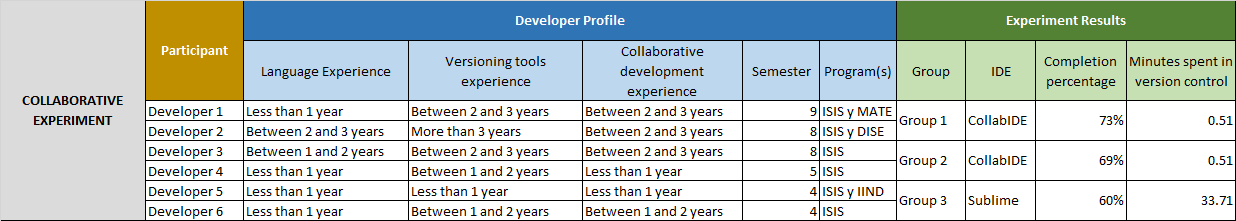
\includegraphics[width=1\textwidth]{img/resultsTableCollaborative}
  \caption{Results for Experiment 1}
  \label{fig:resultsTableCollaborative}
\end{figure}

\subsubsection{Experiment 2 Results}

\fref{fig:resultsTableProductLine} shows the results for each developer. Similar to the first experiment, 
the developers that employed CollabIDE obtained better results, but in this case, the difference 
between using an IDE versus using the other was not very significative. With CollabIDE, the 
developers finished an average of $4\%$ more tasks and spent 
$2.83$ minutes less in version control than the developers using Eclipse.
 The process of creating new product variants and their 
respective functionalities varied significantly in each IDE. With Eclipse and git, participants had to 
create a branch for each variant and then checkout between branches when they needed to work on a 
variant’s specific code. Using CollabIDE, participants needed to first create a product version for each 
variant, then, for each variant create a new developer. This way the participants could take advantage 
of code highlighting and hiding to easily distinguish which code fragments belonged to which variant. 
Thus, while Eclipse and Git make variant creation straightforward, the process of switching between 
them is not as smooth. The contrary happens with CollabIDE, where creating a variant is a longer 
process but switching between them is faster. According to this, it makes sense that in the results 
were close together, as there is a tradeoff when using one IDE over the other. However, in real life 
contexts, projects usually take longer to complete and variant switching operations are more frequent 
than variant creating ones. Therefore, in a real life context CollabIDE could provide better productivity.

When analyzing other factors that could have influenced the experiment, we found one with a potential 
impact on the results. As the tasks needed to be implemented in different languages, the differences 
between these could have led to some developers being more familiar with one of the languages. 
Nevertheless, when we assigned the tasks to each developer we took into account their prior 
experience with the language, so the impact of languages differences may have not been significative

One situation worth mentioning is that one of the developers had problems pushing his changes to 
github, and at the end of the experiment he only had one branch, meaning he lost the changes he 
made to all the other product variants. This occurrence helps reinforce our claim that the use of 
\ac{VCS} can in some cases be detrimental to productivity.

While the results show that CollabIDE does not outperform the other development set-up by a wide 
margin, they do support our second research question up to certain extend. Through the experiment 
the participants were able to effectively generate multiple product variants and switch between them 
with relatively ease, proving that CollabIDE's features are robust enough to enable this type of 
development model.

\begin{figure}[htbp]
  \centering
  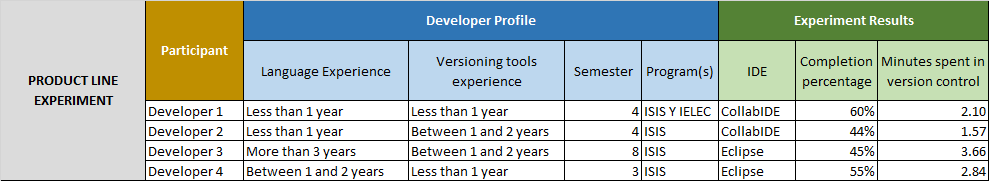
\includegraphics[width=1\textwidth]{img/resultsTableProductLine}
  \caption{Experiment 2 results}
  \label{fig:resultsTableProductLine}
\end{figure}

\subsubsection{Survey}
At the end of the experiment, we asked the participants that used CollabIDE their opinion on the tool's 
main features. All of them agreed that collaborative programming was easy to understand, and of great 
help in completing their tasks. Version management received mixed results as participants thought it 
was not too complex, but not all of them felt this feature helped them during development. Finally, most participants found the product variant management feature useful and easy to use. Overall, 
participants perceived CollabIDE as an intuitive IDE, which let them solve the programming tasks in an 
efficient manner. 

%%%%
\subsection{Threats to Validity}
In this section we discuss some aspects of the experiments that can put at risk the validity of the 
results discussed previously. First, the subject sample size used is small, having only one control group 
in Experiment 1, and two in Experiment 2. Small sample sizes can easily lead to 
bias~\cite{threatstoval}; in this case, the bias would be towards CollabIDE performing better. Another 
aspect that can be considered a threat is the low duration of each experiment. In real life contexts, 
software projects where version control systems are employed usually take weeks to months to 
complete. Additionally, the time intervals between each version control operation are longer, whereas 
in the experiment they needed to be performed each 15 minutes. These lower times could also lead to 
bias towards one of the IDEs, as the development workflow was unfaithful in comparison to those 
carried out in a real life context. 


\endinput
